\section{Глава 2. Алгоритм повышения ОСШ при оценке АКФ}

\subsection{Повышение точности оценки автокорреляционной функции}
Для эффективного использования АР-метода необходимо иметь точную оценку АКФ. Наличие шума в аддитивной смеси ведет к неточной
оценке АКФ, что, в свою очередь, ведет к смещенной оценке резонансных частот. Увеличение ОСШ при вычислении АКФ зависит, в том числе от длительности
выборки. В тех случаях длину выборки увеличить не представляется возможным, например в случае обработки в реальном времени,
возникает необходимость искать другие способы повышения ОСШ.

%%%%%%%%%%%
\subsection{Алгоритм итеративного вычисления АКФ}
\label{sec_ostanin}
В \cite{ostanin_akf} предлагается использовать метод последовательного вычисления АКФ. Данный метод
заключается в последовательном вычислении АКФ от АКФ несколько раз. При этом ОСШ увеличивается от итерации к итерации.
Процесс повторяется несколько раз. Количество итераций зависит от значения ОСШ сигнала. 

Пусть исходный сигнал может быть записан как сумма полезного сигнала ${s(t)}$ и шума ${n(t)}$:
\begin{center}
\begin{equation}
	\label{eq:acf_signal}
	x(t) = A \cos{(\omega t)} + n(t)
\end{equation}
\end{center}

Пусть функции ${s(t)}$ и ${n(t)}$ - центрированы. Тогда АКФ выражения \ref{eq:acf_signal} может быть записан как \cite{book_max}:
\begin{center}
\begin{eqnarray}
	\label{eq:acf_rss_signal}
	r_{xx}(\tau)	& = & \lim_{T \to \infty} \frac{1}{T} \int \limits_0^T x(t)x(t-\tau)dt = \nonumber \\
			& = & \lim_{T \to \infty} \frac{1}{T} \int \limits_0^T (A \cos{(\omega t)} + n(t))(A \cos{(\omega t - \tau)} + n(t - \tau))dt
\end{eqnarray}
\end{center}

Тогда, оценка АКФ может быть записана как:
\begin{center}
\begin{equation}
	\label{eq:acf_rss_signal_full}
	\hat{r}_{xx}(\tau)=\hat{r}_{ss}(\tau)+\hat{r}_{sn}(\tau)+\hat{r}_{ns}(\tau) + \hat{r}_{nn}(\tau)
\end{equation}
\end{center}

Корреляционные функции ${\hat{r}_{xn}}$ и ${\hat{r}_{nx}}$ тождественно равны 0, с точностью до погрешности, при условии независимости
${x(t)}$ и ${n(t)}$. Таким образом \ref{eq:acf_signal} можно переписать:
\begin{center}
\begin{equation}
	\label{eq:acf_rss_signal_new}
	\hat{r}_{xx}(t) = \hat{r}_{ss}(t) + \epsilon (t)
\end{equation}
\end{center}
Стоит учесть, что ${\epsilon (t)}$ стремится к нулю с ростом ${T}$. Фурье-образ ${\hat{r}_{xx}(t)}$
представляет собой СПМ, а следовательно равен квадрату Фурье-образа исходной функции ${x(t)}$.
Если обозначить ОСШ, выраженное в линейных единицах, сигнала ${x(t)}$ как ${R_s}$, тогда ОСШ после вычисления АКФ может быть вычислено
как \cite{book_max}:
\begin{center}
\begin{equation}
	\label{eq:acf_snr_est}
	R_e=2BTR_s \frac{1}{2+1/R_s}
\end{equation}
\end{center}

Стоит отметить, что функция ${\epsilon(\tau)}$, как и ${n(t)}$ - является центрированной и
стационарной случайной величиной.
Учитывая что гармоническая составляющая содержится в ${\hat{r}_{ss}(t)}$, а аддитивный шум в ${\epsilon(\tau)}$, можно провести
следующую итерацию вычисления АКФ. Для оценки ОСШ по формуле \ref{eq:acf_snr_est} нужно принять ${R_s' = R_e}$.

Из \ref{eq:acf_snr_est} видно, что увеличение ОСШ при вычислении оценки АКФ пропорционально ${2BT}$ и зависит от
ОСШ на входе коррелометра, так же можно отметить, что увеличение ОСШ происходит только при условии ${BT > \frac{1}{2R_s} + 1}$.

Так же можно получить оценку АКФ на ${N}$ - шаге. На рисунке \ref{pic:acf_0_iter} представлен входной сигнал, а на
рисунках \ref{pic:acf_1_iter}, \ref{pic:acf_4_iter} представлены оценки АКФ на шагах с 1 и 4.
Моделирование проводилось для гармонического сигнала при ОСШ -44 дБ с нормированной частотой 20 Гц для
отрезка 600 точек.

\begin{figure}[H]
	\center\scalebox{1}{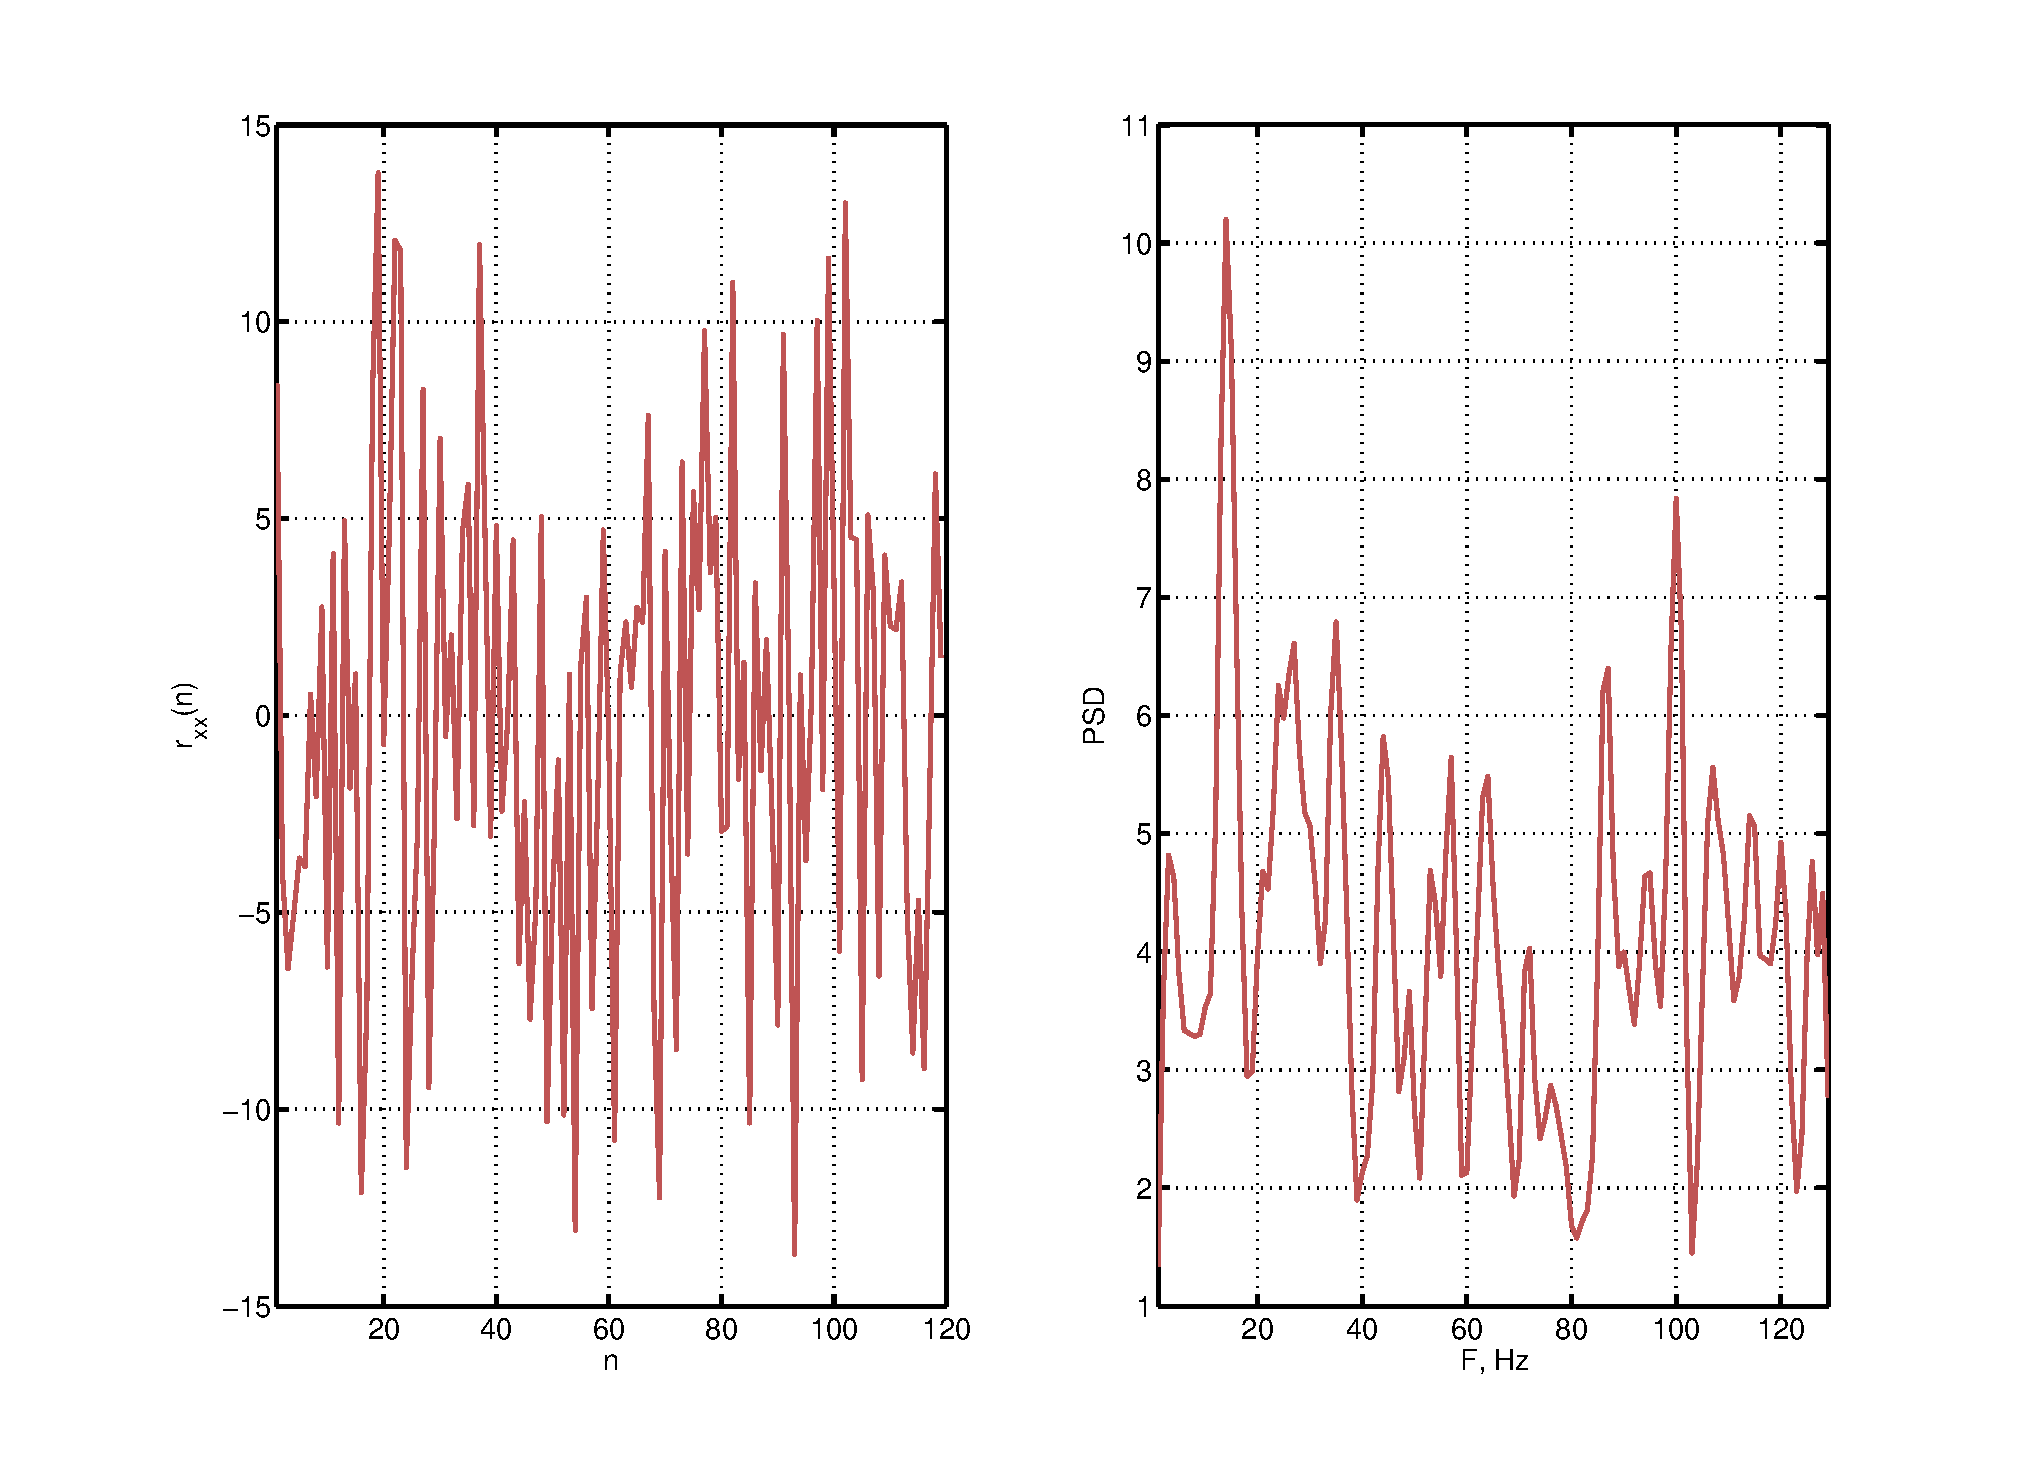
\includegraphics[width=1\linewidth]{acf_0_iter.eps}}
	\caption{Исходный сигнал и его спектр.}
	\label{pic:acf_0_iter}
\end{figure}

\begin{figure}[H]
	\center\scalebox{1}{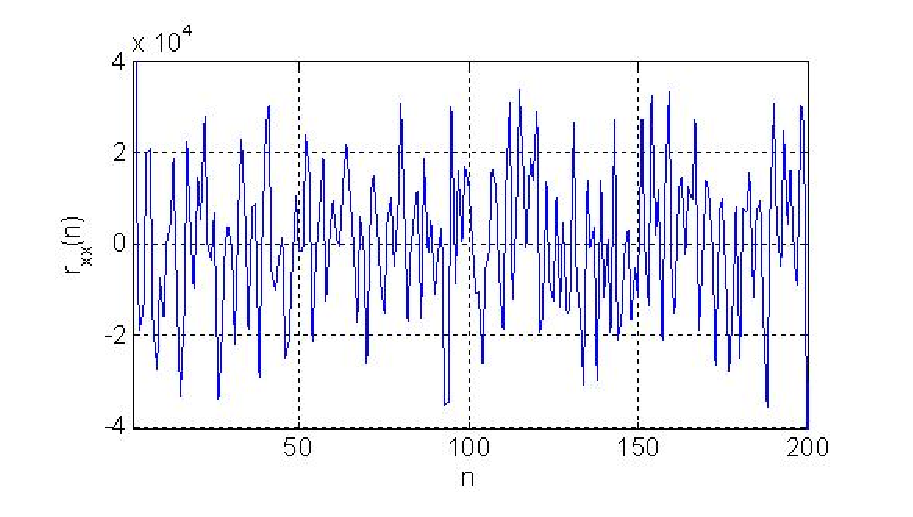
\includegraphics[width=1\linewidth]{acf_1_iter.eps}}
	\caption{Оценка АКФ на 1 итерации и ее спектр.}
	\label{pic:acf_1_iter}
\end{figure}

\begin{figure}[H]
	\center\scalebox{1}{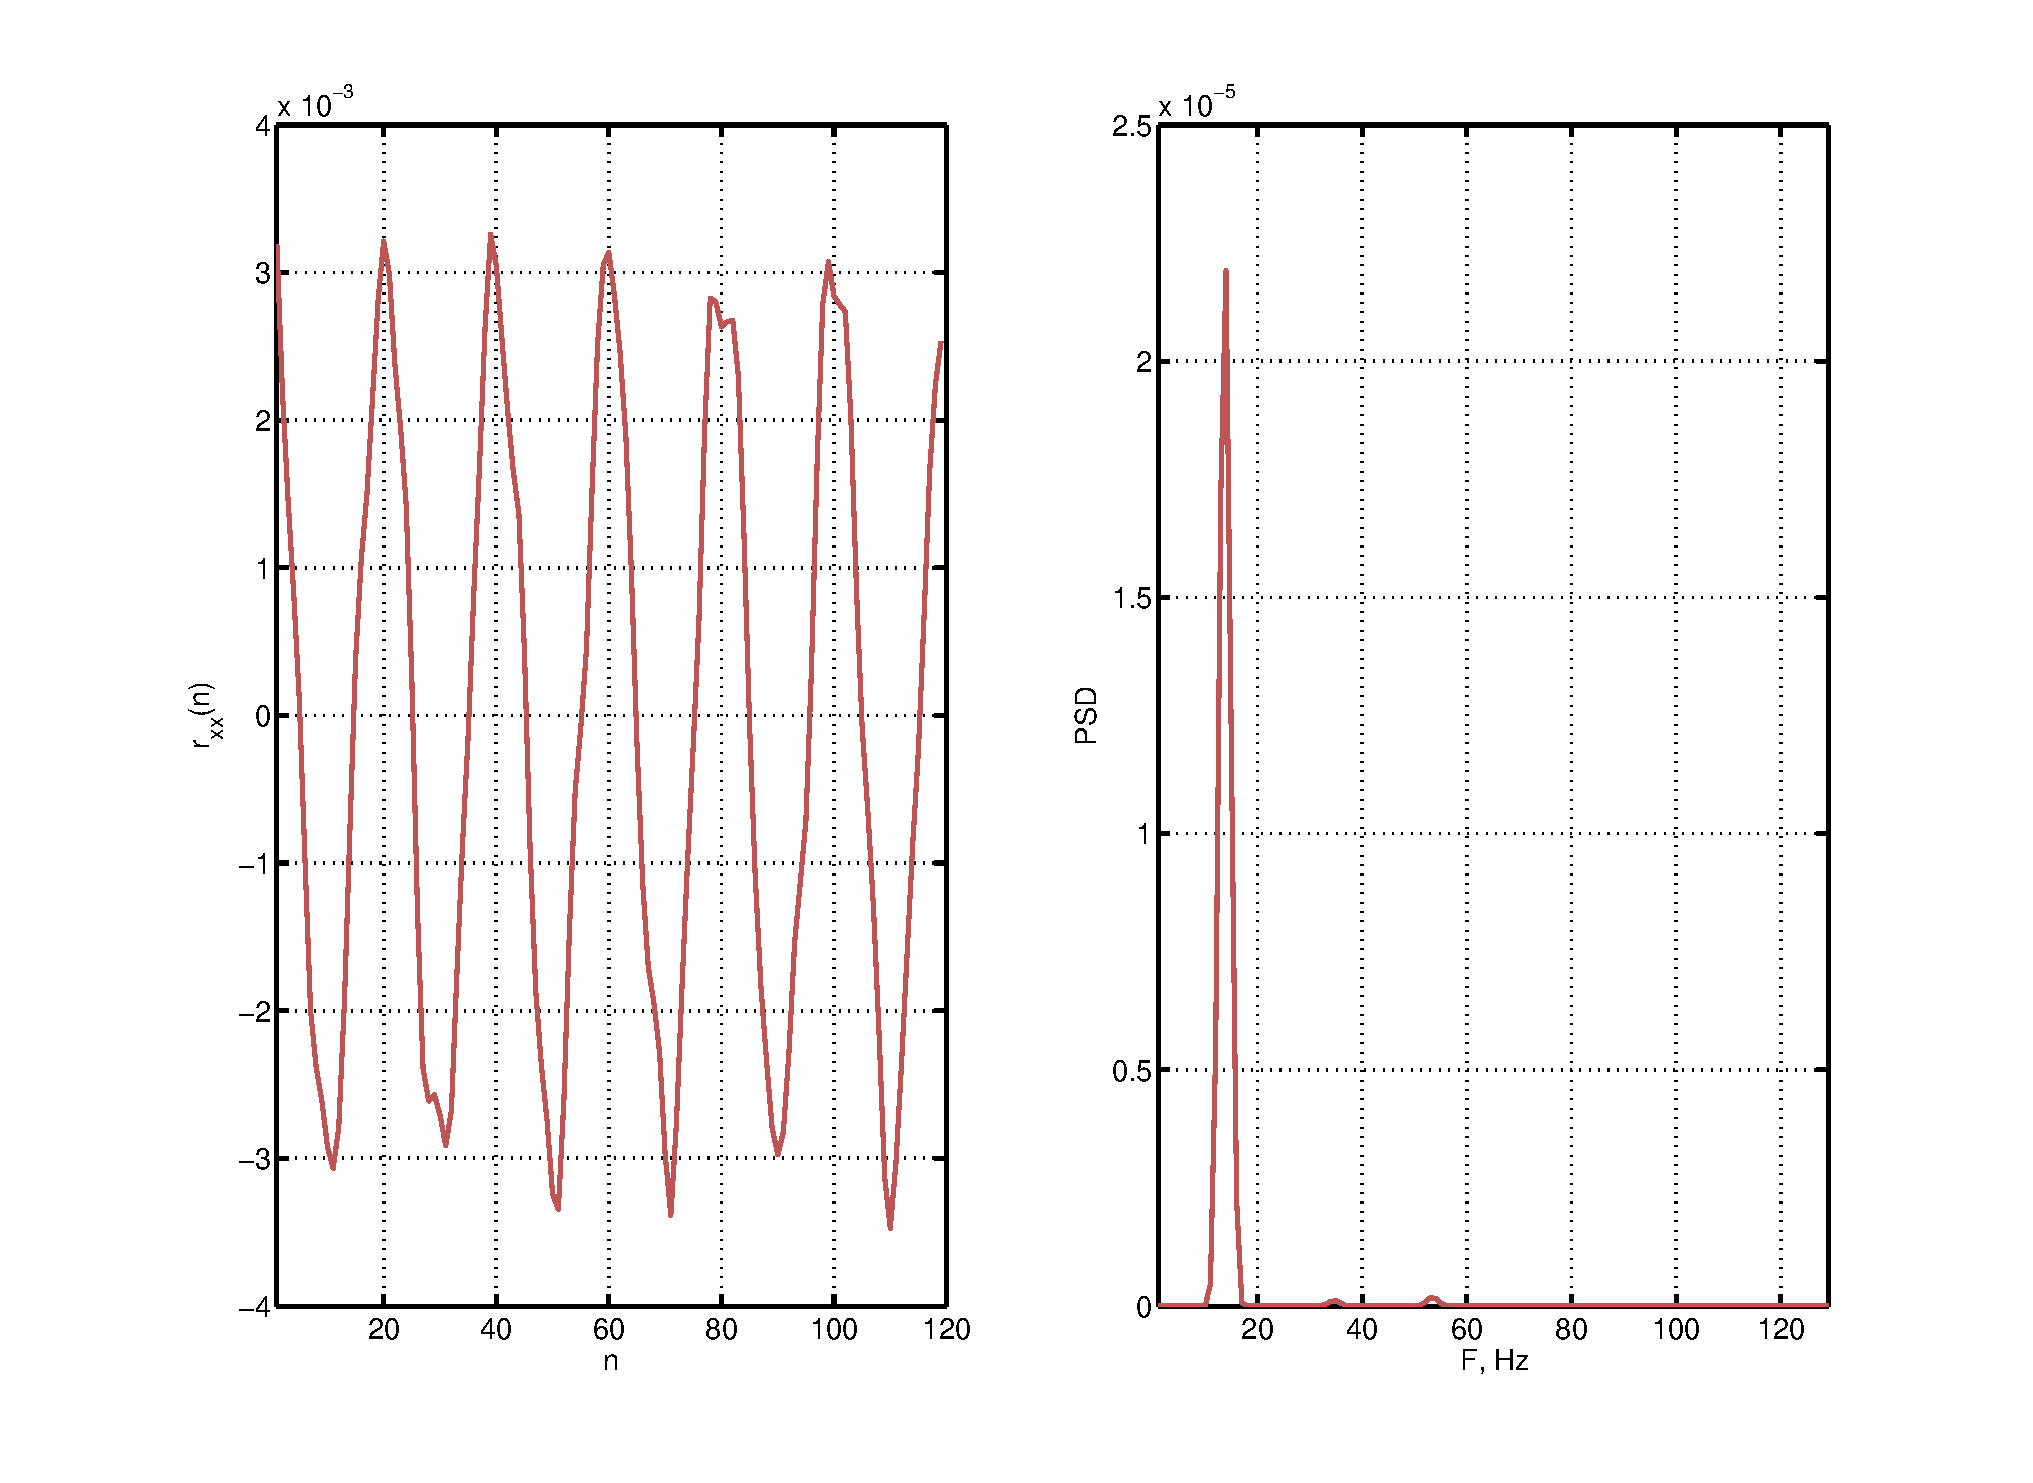
\includegraphics[width=1\linewidth]{acf_4_iter.eps}}
	\caption{Оценка АКФ на 4 итерации и ее спектр.}
	\label{pic:acf_4_iter}
\end{figure}

Представленный алгоритм позволяет значительно улучшить оценку АКФ. Следует отметить, что итеративный алгоритм вычисления АКФ так же
может быть использован для эффективного подавления окрашенного шума. В случае наличия интерференционной помехи в сигнале это дает
возможность получить несмещенную оценку доплеровского сдвига частоты.

%%%%%%%%%%%%%%%%%
\subsection{Усовершенствованный итеративный алгоритм получения АКФ}
\label{sec_acf_fft}
Для приемников реального времени алгоритм, представленный в \cite{ostanin_akf} и приведенный в \ref{sec_ostanin}, применять в алгоритме оценки 
частоты ШПС не представляется возможным в виду большого количества операций при вычислении АКФ.

Автором в \cite{} был предложен способ оптимизации алгоритма последовательного вычисления АКФ.
Для снижения вычислительных затрат указанный алгоритм предлагается реализовывать с использованием процедуры БПФ. 

Посчитаем АКФ для выражения \ref{eq:acf_signal}.
\begin{center}
\begin{equation}
	\label{eq:lpc_akf_n}
	\hat{r}_{xx}(n) = \sum \limits_{k=1}^{K} x(k)x(k+n) = \frac{A^2}{2} \cos{(\omega{n})} + \Delta_n \delta{(n)} + \mu{(n)}
\end{equation}
\end{center}

Здесь ${\Delta_n}$ - дисперсия шума ${n(k)}$, ${\mu{(n)}}$ - ошибка оценки АКФ, ${\delta{(n)}}$ - дельта-функция. Дисперсия ошибки
оценки ${\Delta_{\mu}}$ будет в ${K}$ раз меньше чем дисперсия ${\Delta_n}$ шума в принимаемом сигнале, где ${K}$ - интервал
осреднения оценки АКФ.

Используя оценку АКФ вместо исходной выборки, вновь получим оценку АКФ:
${r_{xx2}(n) = \frac{A^4}{8} \cos{(\omega n)} + \bar{N} \delta{(N)}}$,
где мощность шума оценки ${\bar{N}}$ - будет значительно меньше.

Амплитуда сигнала на итерации ${k}$ будет равна ${\frac{A^{2^k}}{2^{2^k-1}}}$. Увеличение отношения ОСШ по мощности можно
вычислить по уже приведенной формуле \ref{eq:acf_snr_est}. 

В данной работе предложена оптимизированная версия данного алгоритма, позволяющая применять его при обработке сигнала в реальном времени.

Введем следующие обозначения: ${\bf{x}}$ – вектор входного сигнала после снятия ПСП, ${\bf{F}}$ – матрица прямого преобразования Фурье,
${\bf{F}^{-1}}$- матрица обратного преобразования Фурье.  Оценку АКФ на первом шаге можно получить следующим образом:

\begin{center}
\begin{equation}
	\label{eq:akf_1}
	\hat{\bf{r}}_1 = \bf{F}^{-1}\left[ \bf{Fx} \cdot (\bf{Fx})^* \right] = \bf{F}^{-1} \left[ \left| \bf{Fx} \right| ^2 \right]
\end{equation}
\end{center}

Здесь знак ${(\cdot)}$  означает поэлементное перемножение векторов, ${\left| \bf{Fx} \right| ^2}$ - поэлементное возведение модуля комплексного числа в квадрат, ${*}$ -
комплексное сопряжение.  Следуя алгоритму, изложенному в \cite{ostanin_akf} вычислим оценку АКФ от ${\hat{\bf{r}}_1}$:
\begin{center}
\begin{eqnarray}
	\label{eq:akf_2}
	\hat{\bf{r}}_2 & = & \bf{F}^{-1}\left[ \bf{F} \hat{\bf{r}}_1 \cdot (\bf{F} \hat{\bf{r}}_1)^* \right] = \nonumber \\
		& = & \bf{F}^{-1}	\left[ 
				\bf{FF}^{-1} \left[
						\left| \bf{Fx} \right| ^2
					\right]
						\cdot \left( \bf{FF}^{-1} \left[ \left| \bf{Fx} \right| ^2 \right]
					\right) ^*
			\right] = \nonumber \\
		& = & \bf{F}^{-1} \left[ \left| \bf{Fx} \right| ^2 \cdot \left[ \left| \bf{Fx} \right| ^2 \right] ^* \right] =  \nonumber \\
		& = & \bf{F}^{-1} \left[ \left| \bf{Fx} \right| ^4 \right]
\end{eqnarray}
\end{center}

Рассуждая аналогично, можно показать, что уточненная оценка АКФ на ${K}$-ом шаге алгоритма, рассмотренного в \cite{ostanin_akf}
может быть получена без использования итераций с помощью выражения:

\begin{center}
\begin{equation}
	\label{eq:akf_3}
	\hat{\bf{r}}_K = \bf{F}^{-1}\left[ \left| \bf{Fx} \right| ^{2^K} \right]
\end{equation}
\end{center}

Схематически алгоритм получения уточненной оценки АКФ на третьем шаге представлен на рисунке \ref{pic:akf_pic}.

\begin{figure}[H]
	\center\scalebox{0.8}{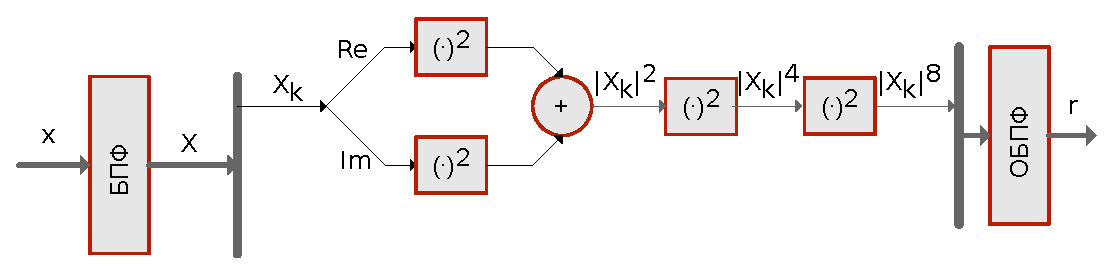
\includegraphics[width=1\linewidth]{akf_fft.eps}}
	\caption{Усовершенствованный итеративный алгоритм получения АКФ}
	\label{pic:akf_pic}
\end{figure}

Количество умножений действительных чисел необходимых для оценки АКФ прямым методом: 
\begin{center}
\begin{equation}
	\label{eq:num_of_op_acf}
	OP_{ACF}=kN^2,
\end{equation}
\end{center}
где ${k}$  – количество итераций.

\begin{enumerate}
\item ${4NlogN}$ - действительных умножений - преобразование Фурье;
\item ${2N}$ - вычисление модуля комплексного числа;
\item ${N}$ - действительных умножений для каждой итерации (возведение в квадрат);
\item ${4NlogN}$ - действительных умножений – обратное преобразование Фурье. 
\end{enumerate}

Окончательно получаем:
\begin{center}
\begin{equation}
	\label{eq:num_of_op_acf}
	OP_{ACF\_FFT}=8NlogN + (k+2)N,
\end{equation}
\end{center}

\subsection{Выводы}

\newpage
